\chapter{高次元エクスパンダー概論}
高次元エクスパンダーとはグラフのエクスパンダー性を単体複体に拡張した概念である.
単体複体上では, 大域的なランダムウォークと局所的なランダムウォークの二つのタイプのランダムウォークを自然に考えることができ, これらに基づいてそれぞれ大域的なエクスパンダー性と局所的なエクスパンダー性の概念が定義できる.
端的に述べると高次元エクスパンダーの理論はこれら二つの概念がほぼ等価であることを明らかにしており, これは単体複体における「局所大域原理」\footnote{局所大域原理(local-global principle)とは整数論などで知られる不定方程式の解の存在性に関して, 局所的な情報が大域的な情報を導くという現象の総称である.}を体現しているといえる.

本チャプターではまず単体複体とその上でのランダムウォークを定義し,
これに基づいて高次元エクスパンダーの定義と重要な性質を紹介する.

\section{定義}
まずは単体複体に関する基礎的な用語を定義していく.
文脈によっては単体複体は多面体などを貼り合わせた幾何的な概念を指すこともあるが,
本講義では組合せ的ないわゆるset system (ハイパーグラフ) としての単体複体を扱う.

\begin{definition}{単体複体}{simplicial complex}
有限集合$V$と$V$の部分集合族$\F\subseteq 2^V$であって部分集合で閉じているもの(すなわち, $\sigma\subseteq \tau \in \F \Rightarrow \sigma\in \F$)の組$X=(V,\F)$を\emph{単体複体 (simplicial complex)}という.
集合族$\F$の元を\emph{面 (face)}と呼び,
面$\sigma \in \F$の\emph{次元 (dimension)}を$\dim \sigma = \abs{\sigma} - 1$とする\footnote{特に, 空集合$\emptyset \in \F$の次元は$-1$である.}.
単体複体$X$の次元を$\dim X = \max\cbra{\dim \sigma \colon \sigma \in \F}$とする.

次元$d$の単体複体$X$は(包含関係に関して)極大な面の次元が全て$d$に等しいとき, \emph{純粋 (pure)}であるという.
整数$-1 \le k \le \dim X$に対し$X(k) = \cbra*{\sigma \in \F\colon \dim \sigma = k }$とする.
特に断りのない限り, $X(0)=V$を仮定する
(そうでなければ$V$として$V=X(0)$とした単体複体を考える).
\end{definition}
面の次元の概念は単体複体の幾何的な表現に由来する.
このイメージになぞらえて,
次元$0$の面を\emph{頂点 (vertex)}, 次元$1$の面を\emph{辺 (edge)}と呼ぶことがある.
次元$2$以上の任意の単体複体$X$に対して$(X(0),X(1))$はグラフである.

\paragraph*{例1.}
グラフ$G=(V,E)$に対し, 空集合, $V$, $E$からなる部分集合族
$\F = \{\emptyset\} \cup \cbra*{\{v\}\colon v \in V} \cup E$考えると,
$(V,\F)$は単体複体である.

\paragraph*{例2.}
有限集合$V$に対し,
$\F = \binom{V}{\le k} \defeq \cbra*{ \sigma \subseteq V \colon |\sigma|\le k}$としたとき, $(V,\mathcal{F})$は純粋な$(k+1)$-次元の単体複体である.

\paragraph*{例3.}
閉路を含まないグラフを\emph{森 (forest)}といい, 連結な森を\emph{木 (tree)}という.
連結グラフ$G$の部分グラフであって木であるものを\emph{全域木 (spanning tree)}という (cf. \cref{def:graph}).
グラフ$G=(V,E)$に対し,
森であるような部分グラフの辺集合からなる集合族$\F\subseteq 2^E$は単体複体である.
すなわち,
\begin{align*}
    \F = \cbra*{ F \subseteq E \colon \text{部分グラフ$(V,F)$は森}}
\end{align*}
に対して$(E,\F)$は単体複体である.
簡単のため$G$を連結グラフであるとすると, $(E,\F)$の極大面は$G$の全域木に対応し, その次元は$n-2$に等しい.
すなわち$(E,\F)$は純粋な$(n-2)$-次元単体複体である.

なお, グラフ$G$が連結でない場合, 異なる連結成分に属する二頂点$u,v$を縮約し一つの頂点として扱うことによって$(V,\F)$の構造を変えないまま連結成分数を減らすことができるので, 連結性を仮定しても一般性を失わない.

\paragraph*{例4.}
実行列$A\in \Real^{n\times m}$ (ただし$m\ge n$) の行ベクトルを$\vec{a}_1,\dots,\vec{a}_n$とする.
集合$V=\{1,\dots,n\}$の部分集合族であって, 線形独立な行ベクトル集合のインデックスとなるものの全体を$\F$とする.
すなわち
\[
    \F = \cbra*{ I \subseteq V\colon (\vec{a}_i)_{i\in I}\text{は線形独立}}
\]
とすると, $(V,\F)$は純粋な単体複体であり, その次元は$A$のランク$\mathrm{rank}(A)$に対し$\mathrm{rank}(A)-1$となる.

\paragraph*{例5.}
部集合$L,R$を持つ二部グラフ$G=(V,E)$を考える.
辺部分集合$M\subseteq E$は, 部分グラフ$(V,M)$の全ての頂点の次数が高々$1$であるとき\emph{マッチング (matching)}という.
マッチング$M$の部分集合$M'\subseteq M$もまたマッチングであるため,
グラフ$G$のマッチング全体からなる辺部分集合族$\F\subseteq 2^E$に対し, $(E,\F)$は単体複体である.
一般に極大マッチングのサイズは異なる場合があるのでこの単体複体は純粋ではない (\cref{fig:matching}).
\begin{figure}[htbp]
    \begin{center}
        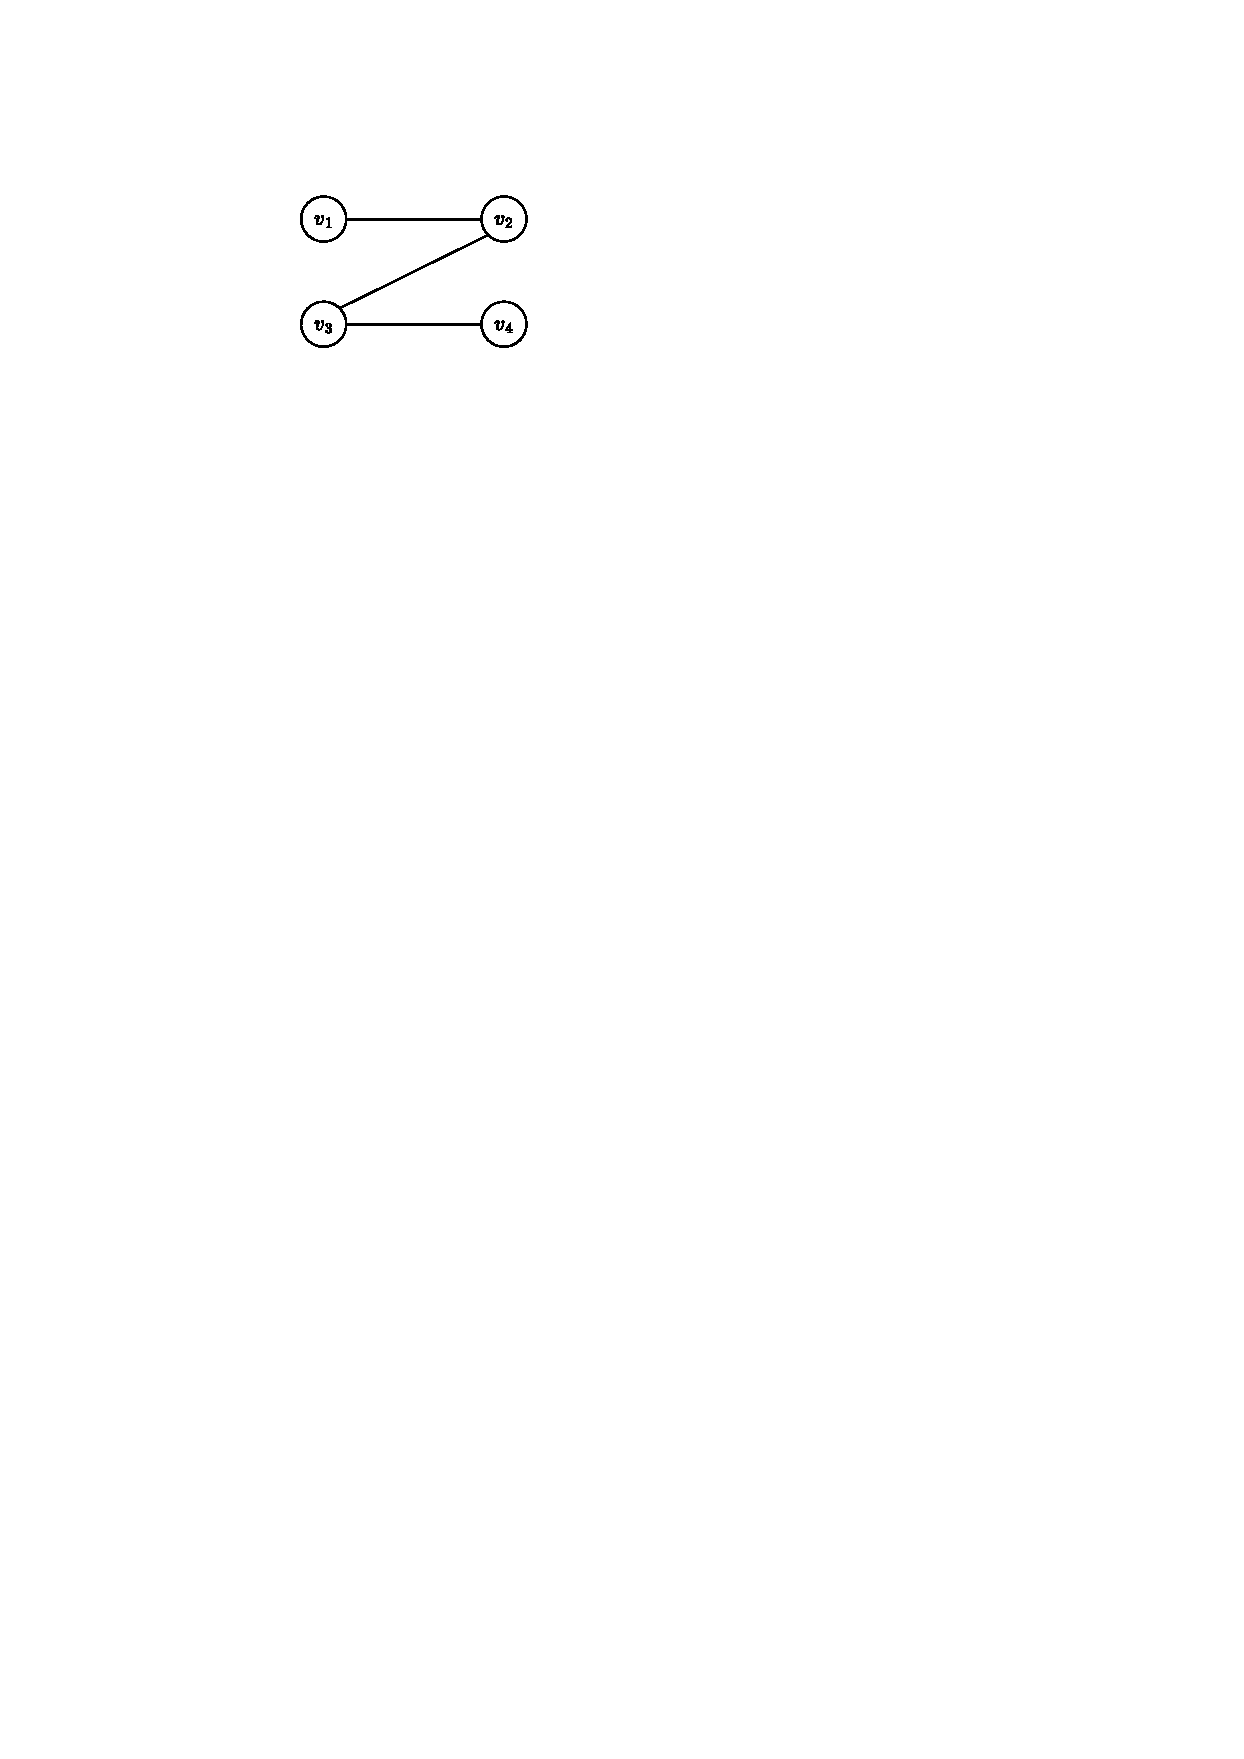
\includegraphics[width=5cm]{images/matching.pdf}
    \end{center}
    \caption{マッチング$M_1=\{v_1,v_2\},\{v_3,v_4\}\}$と$M_2=\{\{v_2,v_3\}\}$はどちらも極大である. \label{fig:matching}}
\end{figure}

\paragraph*{例6.}
グラフ$G=(V,E)$の頂点部分集合$U\subseteq V$は, $U$に属する任意の二頂点間に辺がある(すなわち$\binom{U}{2}\subseteq E$)とき, \emph{クリーク (clique)}\footnote{cliqueとは派閥を意味する英単語である.}という.
特に, 単一頂点からなる集合$\{u\}$や$\emptyset$もクリークである.
クリークの部分集合もまたクリークなので,
グラフ$G$の全てのクリークからなる頂点集合族を$\F$とすると, $(V,\F)$は単体複体である.

\begin{definition}{リンクとスケルトン}{link and skelton}
    単体複体$X=(V,\F)$を考える.
    面$\sigma \in \F$の\emph{リンク (link)}とは単体複体$(V\setminus \sigma, \F_{\sigma})$であって集合族$\F_\sigma$が
    \[
        \F_\sigma = \cbra*{ \tau \setminus \sigma \colon \sigma \subseteq \tau \in \F }
    \]
    で与えられるものである.
    次元$k$以下の面の集合
    \[
        \F_k = \cbra*{ \sigma \in \F \colon \dim \sigma \le k}
    \]
    に対し$(V,\F_k)$を\emph{$k$-スケルトン ($k$-skelton)}という.
\end{definition}
面$\sigma$のリンクとは, $\sigma$をある意味で「縮約」して得られる単体複体であり, 面$\sigma$の周りの局所的な構造を表している.
例えば連結グラフ$G=(V,E)$の森の全体からなる単体複体$X=(E,\F)$を考えよう.
$\sigma\in \F$を一つ固定したとき, リンク$X_\sigma$はどのような単体複体になっているだろうか?
$X_\sigma$の全ての面は辺集合$F$を含むので, $F$に含まれる全ての頂点を縮約して得られるより小さなグラフを考え, そこから$F$の辺を除去して得られるグラフ$G'$の森全体からなる単体複体とみなせる.

%\end{definition}
\section{大域エクスパンダー性}
グラフ上のランダムウォークは頂点集合上で遷移するものを考えていたが,
単体グラフ上のランダムウォークは異なる次元の面の間で遷移するものを考える.
具体的には, \cref{sec:graph up and down walk}で考えたようにある次元$i$の面から次元$i+1$の面に遷移する上昇ウォークと逆に次元$i+1$の面から次元$i$の面に遷移する下降ウォークである.
上昇ウォークと下降ウォークが互いに随伴の関係になるようにするため, 各$X(i)$上での定常分布を定義し, $X(i)$と$X(i+1)$の間で詳細釣り合い条件が満たされるように定義される.

\subsection{下降ウォークと定常分布}
まず, \cref{sec:graph up and down walk}で考えた下降ウォークを単体複体に拡張し, $X(d-1)$上では一様分布を定常分布とすることによって帰納的に各$X(i)$上での定常分布を定める.
\begin{definition}{下降ウォークと面上の定常分布}{down walk and stationary distribution}
    純粋な$d$次単体複体$X=(V,\F)$を考える.
    各$i=0,\dots,d-1$に対し
        確率行列$\Pdown_i \in [0,1]^{X(i) \times X(i-1)}$を
        \[
            \Pdown_i(\tau,\sigma) = \begin{cases}
                \frac{1}{i+1}	& \tif \sigma \subseteq \tau,\\
                0 & \totherwise
            \end{cases}
        \]
        とする.
    各$i=0,\dots,d-1$に対して, $X(i)$上の分布$\pi_i \in [0,1]^{X(i)}$を
        \begin{itemize}
        \item $i=d-1$のとき, $\pi_{d-1}$は$X(d-1)$上の一様分布. すなわち$\pi_{d-1}(\sigma) = \frac{1}{\abs{X(d-1)}}$
        \item $\pi_{i+1}$が定義されているとき, $\pi_i = \pi_{i+1}\Pdown_{i+1}$
        \end{itemize}
    で定める.
    分布$\pi_i$を($i$次の)定常分布と呼ぶ.
\end{definition}
面$\tau \in X(i+1)$に対して$\Pdown_{i+1}(\tau,\cdot)$で定まる$X(i)$上の分布は, 面$\tau$に含まれる頂点$u$を一様ランダムに選んだときの$\sigma = \tau \setminus\{u\}$の分布と等しい.
この分布は, まず一様ランダムに$X(d)$から面を選び, その中から一様ランダムに選ばれた$i+1$個の頂点からなる$X(i)$の面のなす分布である.
特に全ての$\sigma\in X(i)$に対し$\pi_i(\sigma)=0$である
(そうでなければ, $\pi_d$が一様分布であることに反する).
ある面$\tau\in X(i+1)$から分布$\Pdown_{i+1}(\tau,\cdot)$に従ってランダムに選ばれた面$\sigma$に遷移する過程を\emph{下降ウォーク (down walk)}と呼ぶ.

\subsection{上昇ウォーク}
\cref{def:down walk and stationary distribution}では次元$i$の面から次元$i-1$に遷移する下降ウォークを与えた.
同様に, 次元$i$の面から次元$i+1$の面に遷移する上昇ウォークを, $X(i)$と$X(i+1)$の間の詳細釣り合い条件が成り立つように定義する.
%
\begin{definition}{上昇ウォーク}{up walk}
    純粋な$d$次単体複体$X=(V,\F)$を考える.
    各$i=-1,\dots,d-2$に対し
        確率行列$\Pup_i \in [0,1]^{X(i) \times X(i+1)}$を
    \begin{align*}
        \Pup_i(\sigma,\tau) &= \frac{\pi_{i+1}(\tau)}{\pi_i(\sigma)}\Pdown_{i+1}(\tau,\sigma) \\
        &= \begin{cases}
            \frac{\pi_{i+1}(\tau)}{(i+1)\pi_i(\sigma)}	& \tif \sigma\subseteq \tau,\\
            0 & \totherwise
        \end{cases}
    \end{align*}
    で定める.
\end{definition}
%
二つの面集合$X(i)$と$X(i+1)$を部集合とする二部グラフを考えればわかりやすい.
それぞれの部集合には$\pi_i,\pi_{i+1}$が定常分布として付随しており,
上昇ウォーク$\Pup_i$と下降ウォーク$\Pdown_{i+1}$は詳細釣り合い条件
\[
    \forall \sigma\in X(i),\tau\in X(i+1),\,\pi_i(\sigma)\Pup_i(\sigma,\tau) = \pi_{i+1}(\tau)\Pdown_{i+1}(\tau,\sigma)
\]
を満たしている.

なお, 下降ウォーク$\Pdown_{i}$と上昇ウォーク$\Pup_i$の添字$i$は遷移の開始地点の面の次元としている.
%
    各$X(i)$に対して空間$\ell^2_{\pi_i}(X(i))$, 
    すなわち, \cref{def:naiseki}と同様にして$\Real^{X(i)}$に内積$\abra{\cdot,\cdot}_{\pi_i}$が導入された空間を定義できる.
    このとき, 
    \[\Pup_i\colon \ell^2_{\pi_{i+1}}(X(i+1)) \to \ell^2_{\pi_{i}}(X(i))\]
    と
    \[\Pdown_{i+1}\colon \ell^2_{\pi_{i}}(X(i)) \to \ell^2_{\pi_{i+1}}(X(i+1))\]
    は互いに随伴の関係にある.
    すなわち, 任意の$f\in \ell^2_{\pi_i}(X(i)),g\in \ell^2_{\pi_{i+1}}(X(i+1))$に対して
    \begin{align} \abra{\Pup_i f, g}_{\pi_{i+1}} = \abra{ f,\Pdown_{i+1}g }_{\pi_i} \label{eq:adjoint up and walk}\end{align}
    が成り立つ.
%
\begin{exercise}{}{adjoint check}
    \cref{eq:adjoint up and walk}を確認せよ.
    すなわち, \cref{def:down walk and stationary distribution}で定義された定常分布$\pi_i,\pi_{i+1}$および任意の二つの関数$f\colon X(i) \to \Real,g\colon X(i+1) \to \Real$に対して
    \[ \sum_{\sigma \in X(i)} \pi_i(\sigma) f(u) = \sum_{\tau \in X(i+1)} \pi_{i+1}(\tau) g(\tau) \]
を確認せよ.
\end{exercise}

最後に, 上昇ウォークと下降ウォークを組み合わせることによって面$X(i)$上の2種類のランダムウォークが定義できる:
\begin{definition}{上昇下降と下降上昇ウォーク}{UD and DU walk}
    \cref{def:down walk and stationary distribution}, \ref{def:up walk}と同じ設定を考える.
    \begin{align*}
        &\PUD_i \defeq  \Pup_i \Pdown_{i+1},\\
        &\PDU_i \defeq \Pdown_{i}\Pup_{i-1}
    \end{align*}
    を遷移確率行列として持つ$X(i)$上のランダムウォークをそれぞれ\emph{上昇下降ウォーク (up-down walk), 下降上昇ウォーク (down-up walk)}と呼ぶ.
    ここで, $X(-1)$上での下降上昇ウォークと$X(d-1)$上での上昇下降ウォークは定義されない.
\end{definition}
上昇下降ウォークはグラフ上の遅延単純ランダムウォークの自然な一般化になっている (\cref{sec:graph up and down walk}).
\begin{lemma}{定常分布}{UP and DU stationary distribution}
    面$X(i)$上の上昇下降ウォークと下降上昇ウォークはどちらも$\pi_i$を定常分布としてもつ.
\end{lemma}
\begin{proof}
    計算によって簡単に確認できる.
    実際,
    \begin{align*}
        &\pi_i \PUD_i = \pi_i \Pup_i \Pdown_{i+1} = \pi_{i+1} \Pdown_{i+1} = \pi_i, \\
        &\pi_i \PDU_i = \pi_i \Pdown_i \Pup_{i-1} = \pi_{i-1}\Pup_{i-1} = \pi_i
    \end{align*}
    より主張を得る.
\end{proof}
\begin{remark}{「上昇」「下降」の名称}{up and down}
    非常にややこしいのだが,
    上昇ウォークと下降ウォークの遷移確率行列と左右どちらから作用させるかによって「上昇」「下降」の意味合いが反転してしまう.
    確率行列としての上昇ウォークは$\Pup_i \in [0,1]^{X(i)\times X(i+1)}$で表せる.
    一般によくある左から作用させる作用素の感覚で考えると
    $\Pup_i\colon \Real^{X(i+1)} \to \Real^{X(i)}$
    であるので, 次元を一つ落とすように見えてしまうのである.
    下降ウォークについても同様である.
    特に上昇下降ウォーク$\PUD_i=\Pup_i\Pdown_{i+1}$を左から作用させると「次元を下げてから上げる」ものになるので, 下降上昇ウォークと混同しやすい.
    
    本講義はランダムウォークを主眼におき, 右から作用させるときの$\Pup_i,\Pdown_i$に興味があるので, 左固有値以外の文脈ではとにかくランダムウォークの遷移確率行列といえば右から作用させるものであると考えていき, 名称についても
    \cref{def:down walk and stationary distribution}, \ref{def:up walk}の呼称を採用している.
    
    そもそも, 遷移確率行列$P(u,v)$を「$u$から$v$に遷移する確率」として定義してしまったのが根本的な原因であり, 転置したものを改めて遷移確率行列と定義しなおせば解決できるのだが, ランダムウォークの文化ではもはや\cref{def:random walk}の定義が完全に主流となってしまっておりそれに反するとほとんどの参考文献が読みづらくなってしまうので従った.
    
    なお, 可逆なランダムウォーク(\cref{def:reversible})は内積$\piprod{\cdot,\cdot}$の意味で左右どちらから作用させても本質的に同じであるので左右どちらから作用させるかについてこのような煩雑な話は考えなくて良い.
\end{remark}

\section{局所エクスパンダー性}
単体複体の各リンクに対して局所的なランダムウォークを次のように定義する.
\subsection{局所的なランダムウォーク}
全てのリンクの$2$-スケルトン上での局所的な重み付きランダムウォークを考える.
重み付きランダムウォークについては\cref{def:weighted random walk}を参照されたい.
%
\begin{definition}{局所ランダムウォーク}{local random walk}
    純粋な$d$次元単体複体$X = (V,\F)$を考える.
    次元$i \le d-2$の面$\sigma \in \F$に対し,
        リンク$X_\sigma$の$2$-スケルトンを$G_\sigma = (V_\sigma,E_\sigma)$とする.
    このグラフの辺重み$w_\sigma\colon E_\sigma \to [0,1]$を
    \[ w_\sigma(e) = \pi_i(\sigma\cup e) \]
    で定め, これによって定まる$V_\sigma$上の重み付きランダムウォークを面$\sigma$に関する\emph{局所ランダムウォーク (local random walk)}と呼び\footnote{このランダムウォークの概念は高次元エクスパンダーの文脈ではほぼ必ず登場するが, 特に標準的な用語が与えられてはいないので、「局所ランダムウォーク」という用語は本講義だけの局所的なものとする.}, 遷移確率行列を$P_\sigma\in [0,1]^{V_\sigma\times V_\sigma}$とする.
\end{definition}
%
必ずしも局所ランダムウォークが既約性や非周期性を持つとは限らない(すなわち, グラフ$G_\sigma$が非連結だったり二部グラフになりうる)が,
可逆性は必ず満たすことに注意せよ.

グラフ($1$次元単体複体)だと面$\emptyset$に対する局所ランダムウォークのみ存在するが, これは上昇下降ウォーク(すなわち遅延単純ランダムウォーク)と同じである.
従って局所ランダムウォークの概念はより高次元の単体複体を考える際に意味を持つ.

%
\begin{lemma}{}{local random walk stationary distribution}
    遷移確率行列$P_\sigma$をもつ局所ランダムウォークの定常分布を$\pi_\sigma$とすると, 
\end{lemma}
%
\subsection{局所エクスパンダー}
純粋な単体複体の局所的なエクスパンダー性を定義する.
任意の面$\sigma$に対し$G_\sigma$上での局所ランダムウォークの第二固有値が小さいとき, その単体複体は局所的エクスパンダー性をもつという.
\begin{definition}{局所エクスパンダー性}{local expander}
    純粋な$d$次元単体複体$X=(V,\F)$は,
    任意の面$\sigma\in\F$に対し$\lambda_2(P)\le \lambda$を満たすとき,
    \emph{局所$\lambda$-エクスパンダー (local $\lambda$-expander)}であるという.
    より一般に, 任意の$i=-1,\dots,d-2$と任意の面$\sigma\in X(i)$に対して$\lambda_2(P_\sigma) \le \lambda_i$を満たすとき, 単体複体$X$は局所$(\lambda_{-1},\dots,\lambda_{d-2})$-エクスパンダーであるという.
\end{definition}
エクスパンダーグラフ(\cref{def:expander})と比較すると, 片側($\lambda_2$)だけの上界だけでエクスパンダー性を定義している.
これは, 単体複体上の上昇下降ウォークがグラフ上の遅延単純ランダムウォークに対応していることに起因する (遅延単純ランダムウォークの遷移確率行列は半正定値だから$\lambda_2$の上界だけあれば混交性が保証される).
%

\section{Oppenheimのトリクルダウン定理}

\section{高次元エクスパンダーの応用}
理論計算機科学における高次元エクスパンダーの応用を簡単にまとめる.
特にマトロイドに関するものは次チャプターにて解説する.
本質的には,
局所的な情報(局所ランダムウォークの混交性)が大域的な情報(上昇下降ランダムウォークの混交性)を導出するという性質が極めて重要であり,
これに基づいて誤り訂正符号などの構成がなされている.